\documentclass[notitlepage, a4paper, 11pt]{article}

\usepackage{geometry}
\geometry{
	a4paper,
	total={170mm,257mm},
	left=20mm,
	top=20mm,
}

\usepackage{ gensymb }
\usepackage{wrapfig}
\usepackage{xcolor}
\usepackage{graphicx}
\usepackage{amsmath}
\usepackage{listings}
\usepackage{xcolor}
\usepackage{minted}
\usepackage{tikz}
\usepackage[european resistors]{circuitikz}
\usepackage{caption}
\usepackage{subcaption}
\usepackage{hyperref}
\hypersetup{
	pdfborder = false,
	colorlinks=true,
	linkcolor=black,
	filecolor=black,      
	urlcolor=blue,
	pdftitle={Overleaf Example},
	pdfpagemode=FullScreen,
}
\title{Frequency Response Measurements\\
	\large Laboratory VI}
\author{Patrycja Nazim, Adrian Król, Gabriel Ćwiek, Kamil Chaj}
\date{}

\begin{document}
	\maketitle
	\section{Goal of the exercise}
	\section{Frequency response}
	\section{Course of measurements}
	\begin{figure}[H]
		\centering
		\begin{circuitikz}[scale = 0.7, transform shape]
			\draw (0,0) node[bnc](B1) {CON11}
			to[R, l=$R_{11}$, a=1.5k$\Omega$] (3,0)
			to[C, l=$C_{11}$, a=47nF] (3,-2)
			node[ground] {}
			;
			\draw (3,0) 
			to[short] (4.5,0)
			node[bnc, xscale=-1](B2){\scalebox{-1}[1]{CON12}}
			;
			\draw node[ground] at (B1.shield) {};
			\draw node[ground] at (B2.shield) {};
		\end{circuitikz}
	\end{figure}
	\section{Data processing}
	\section{Characteristics analysis}
	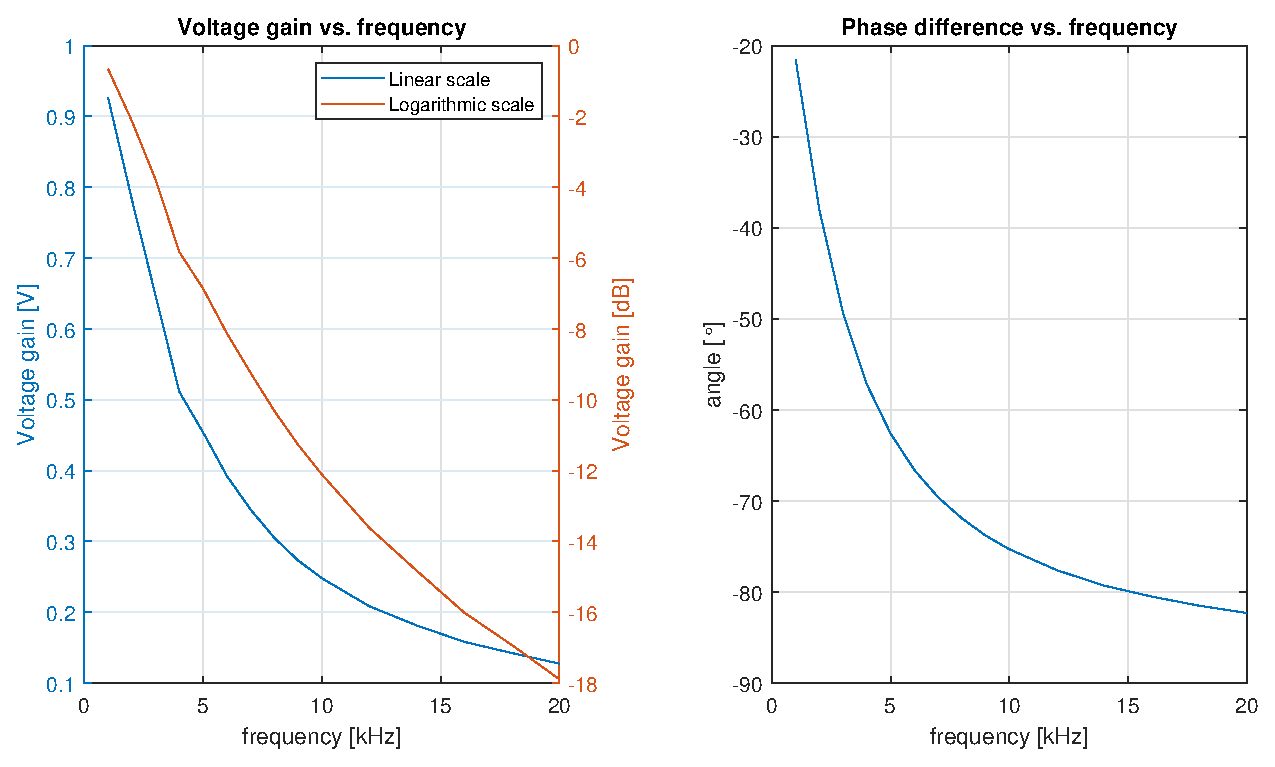
\includegraphics[width=\textwidth]{../Matlab/img/11.eps}
	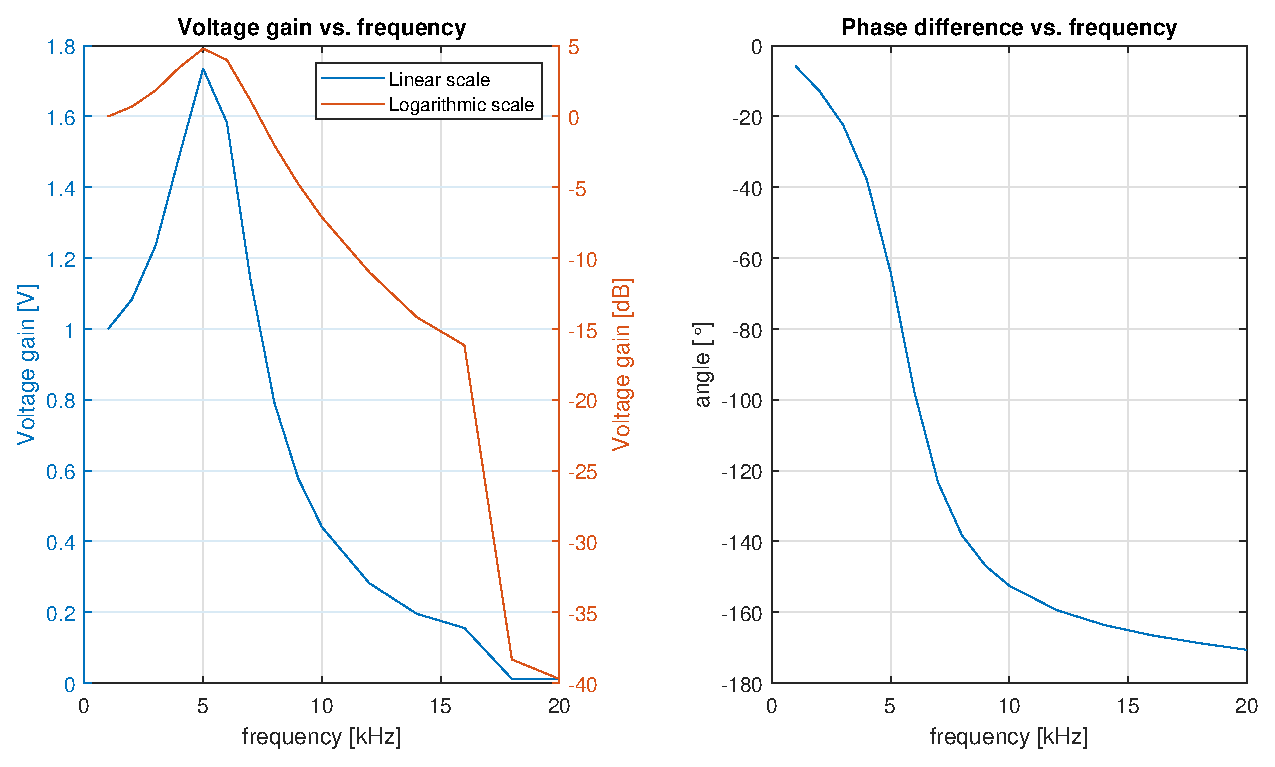
\includegraphics[width=\textwidth]{../Matlab/img/12.eps}
	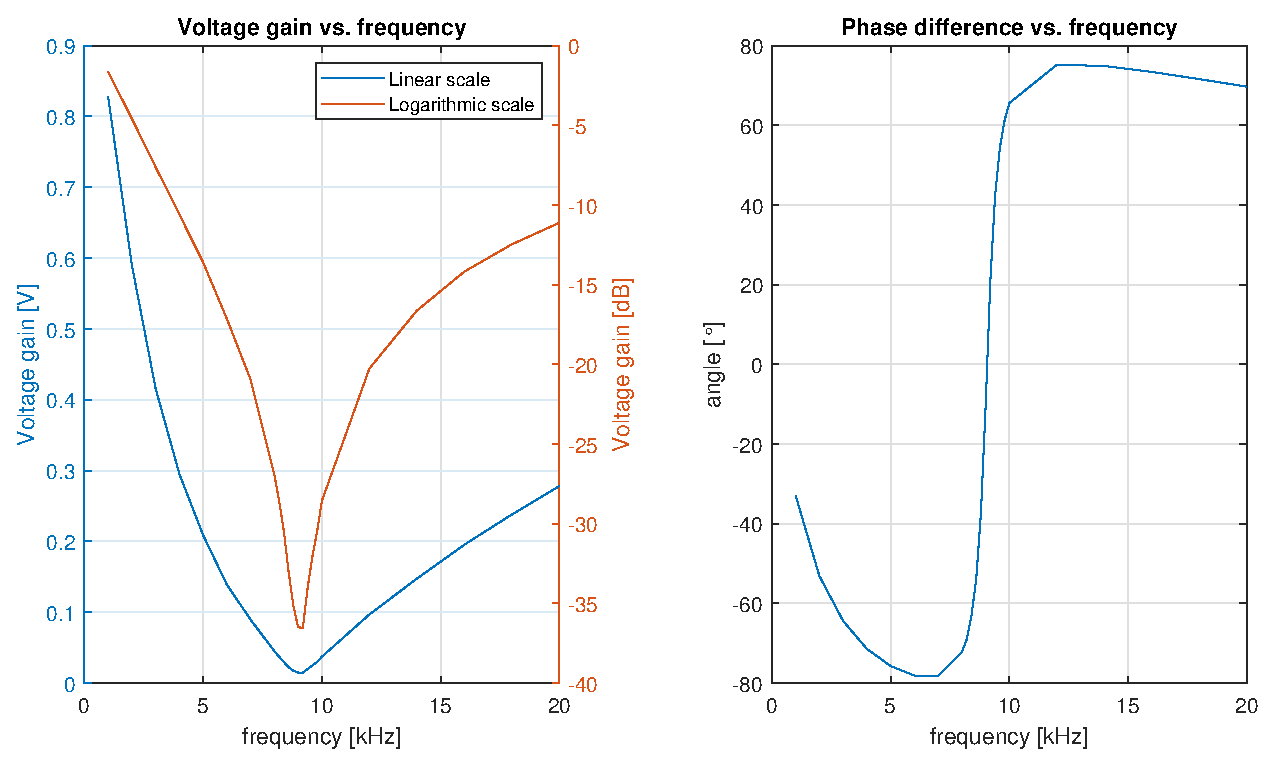
\includegraphics[width=\textwidth]{../Matlab/img/131.eps}
	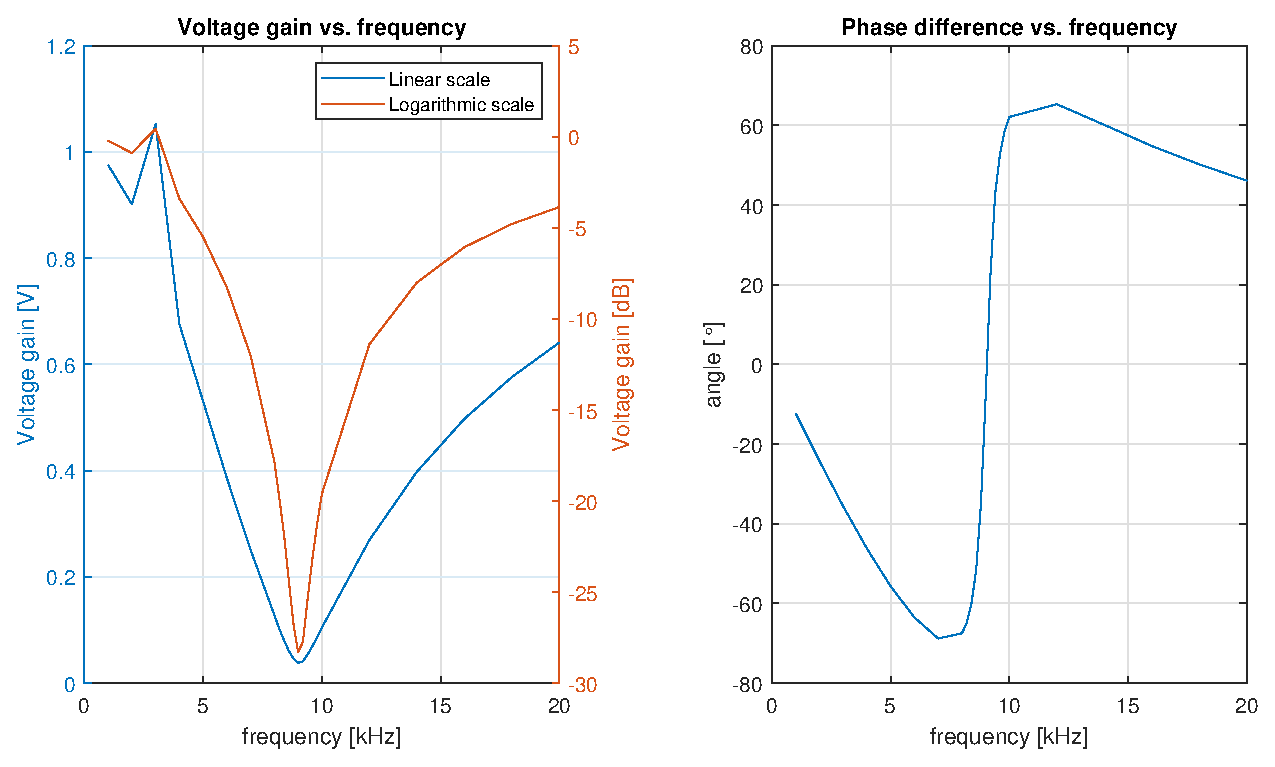
\includegraphics[width=\textwidth]{../Matlab/img/132.eps}
	\section{Conclusions}
\end{document}